\documentclass[aspectratio=169,11pt]{beamer}

\usetheme{metropolis}
\usepackage{booktabs}
\usepackage{graphicx}
\graphicspath{{../report/figures/}{../report/images/}}

\metroset{block=fill}

\title{Laser Radius Sensor Selection}
\subtitle{EVKA Spherical Positioning System --- Requirement Study}
\author{EVKA Position Project}
\date{2026-07-01}

\begin{document}

\maketitle

% ---------------------------------------------------------------
\begin{frame}{Requirement \& Scope}
  \textbf{Only the radius source changes.} Two rotary encoders (Autonics E40S6,
  20\,000 PPR) keep measuring $\theta$ and $\phi$ --- unchanged. The draw-wire is
  replaced by a laser distance reading for $r$.
  \vspace{0.6em}

  \begin{block}{Fixed requirement (confirmed with project owner)}
    \begin{itemize}
      \item Range: \textbf{$\leq$ 40 m}
      \item Laser device accuracy: \textbf{$\leq$ 10 mm} (target sub-cm) across full range
      \item This is the \emph{device datasheet spec} --- a selection filter, not total XYZ accuracy
    \end{itemize}
  \end{block}
  \vspace{0.3em}

  \begin{columns}[t]
    \column{0.5\textwidth}
    \textbf{Version A} --- detachable handheld, docked on the phi head; quick-disconnect for field use.
    \column{0.5\textwidth}
    \textbf{Version B} --- permanently mounted fixed module; automation-first, no handling.
  \end{columns}
\end{frame}

% ---------------------------------------------------------------
\begin{frame}{Why Phase-Shift, Not Pulsed Time-of-Flight}
  \textbf{Pulsed ToF} (Benewake TF-series, DFRobot) --- times a light pulse
  directly $\rightarrow$ \alert{$\pm$5 cm to $\pm$1\% of reading}.
  \textbf{Fails the spec}, excluded.
  \vspace{1em}

  \textbf{Phase-shift / AMCW} (Leica, Meskernel, Dimetix) --- measures beam
  phase $\rightarrow$ \textbf{flat $\pm$1--2 mm} at any range.
  Every \textbf{certified} device is phase-shift; Bosch \& JRT are
  \alert{flagged} --- principle unconfirmed (2026-07-08).
\end{frame}

\begin{frame}{Accuracy vs.\ Range --- $\leq$10 mm Requirement}
  \centering
  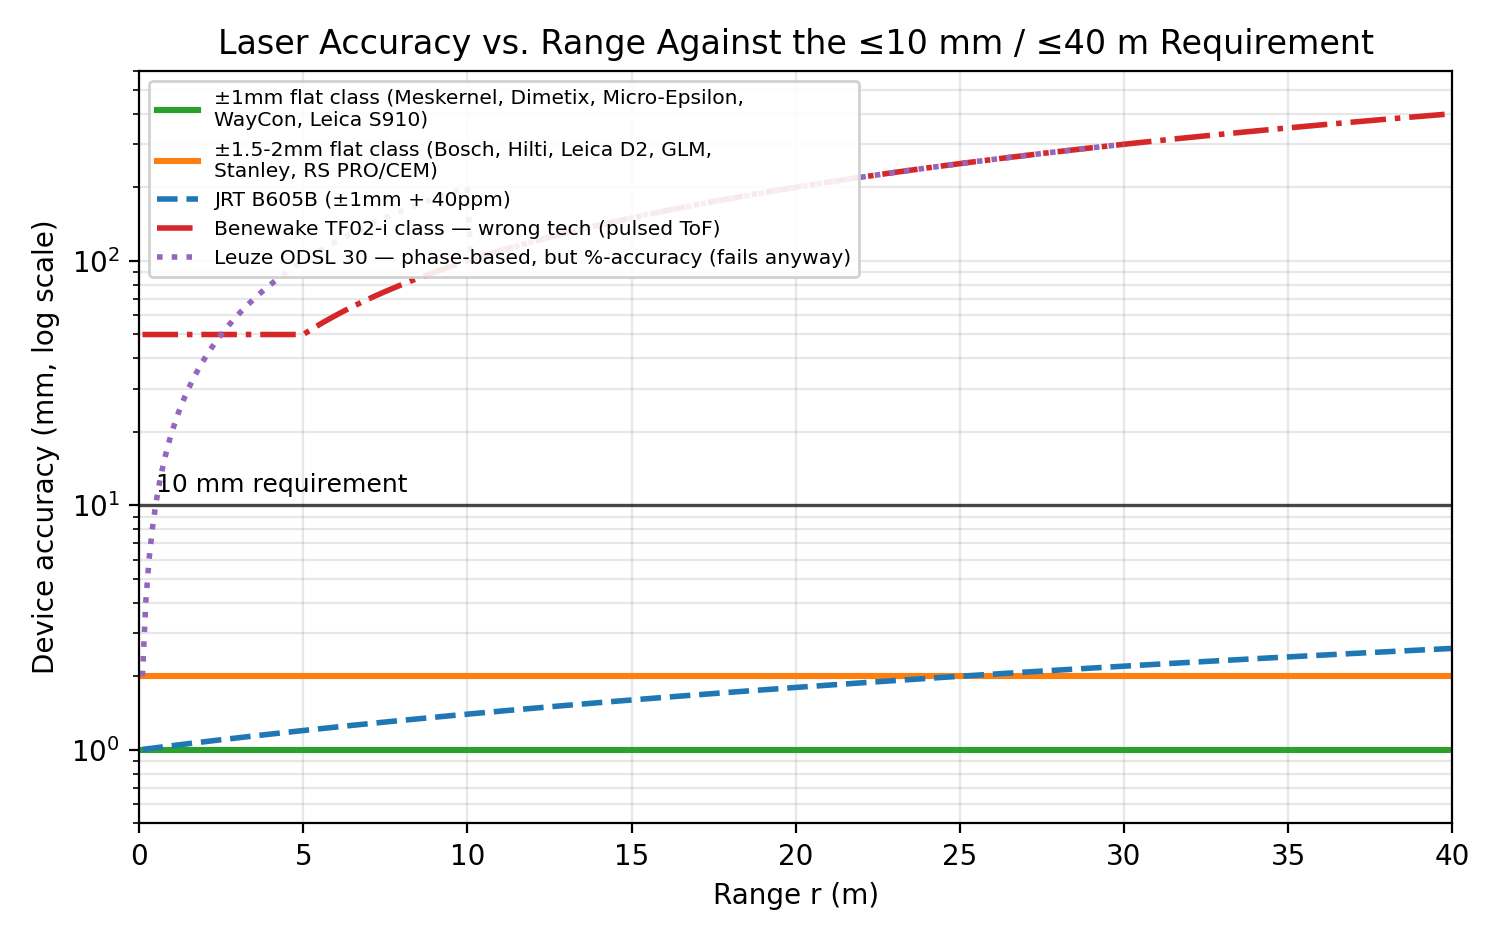
\includegraphics[height=0.82\textheight]{accuracy_vs_range.png}
\end{frame}

% ---------------------------------------------------------------
\begin{frame}{Device Shortlist (meets $\leq$40 m / $\leq$10 mm)}
  \centering
  \footnotesize
  \begin{tabular}{@{}lllll@{}}
    \toprule
    \textbf{Device} & \textbf{Range} & \textbf{Accuracy} & \textbf{Interface} & \textbf{Price} \\
    \midrule
    Meskernel LDL-T      & 0.03--80 m  & $\pm$1 mm, 100 Hz        & RS232/485/USART   & \$87.50 \textbf{c.} \\
    Dimetix DBN-50-050   & 0.05--50 m  & $\pm$5 mm, \textbf{pub.\ ASCII} & RS232 / RS422     & \$1{,}332 \textbf{c.} \\
    Leica DISTO D5       & 0.05--200 m & $\pm$1.0 mm              & BLE 5.0 + USB-C   & \$311--708 \textbf{c.} \\
    Leica DISTO S910     & 0.05--300 m & $\pm$1.0 mm              & BLE + native USB  & \$1{,}916--2{,}132 \textbf{c.} \\
    Bosch PLR 40 C$^\dagger$  & 0.05--40 m  & $\pm$2 mm                & BLE 4.2           & \$110--125 \\
    JRT B605B$^\dagger$       & 0.03--150 m & $\approx\pm$2.6 mm @ 40 m & RS232 TTL         & \$43--90 \\
    \bottomrule
  \end{tabular}
  \vspace{0.6em}

  \scriptsize \textbf{c.} = confirmed price (2026-07-08 survey). \quad
  $^\dagger$ = phase-shift principle \alert{unconfirmed} --- held out of the certified list.
  \vspace{0.4em}

  \normalsize
  20 qualifying/flagged devices total. Accuracy is never the problem;
  \textbf{price, sourcing, and interface} are the real decisions.
\end{frame}

\begin{frame}{Price vs.\ Accuracy --- You Pay for Housing, Not Accuracy}
  \centering
  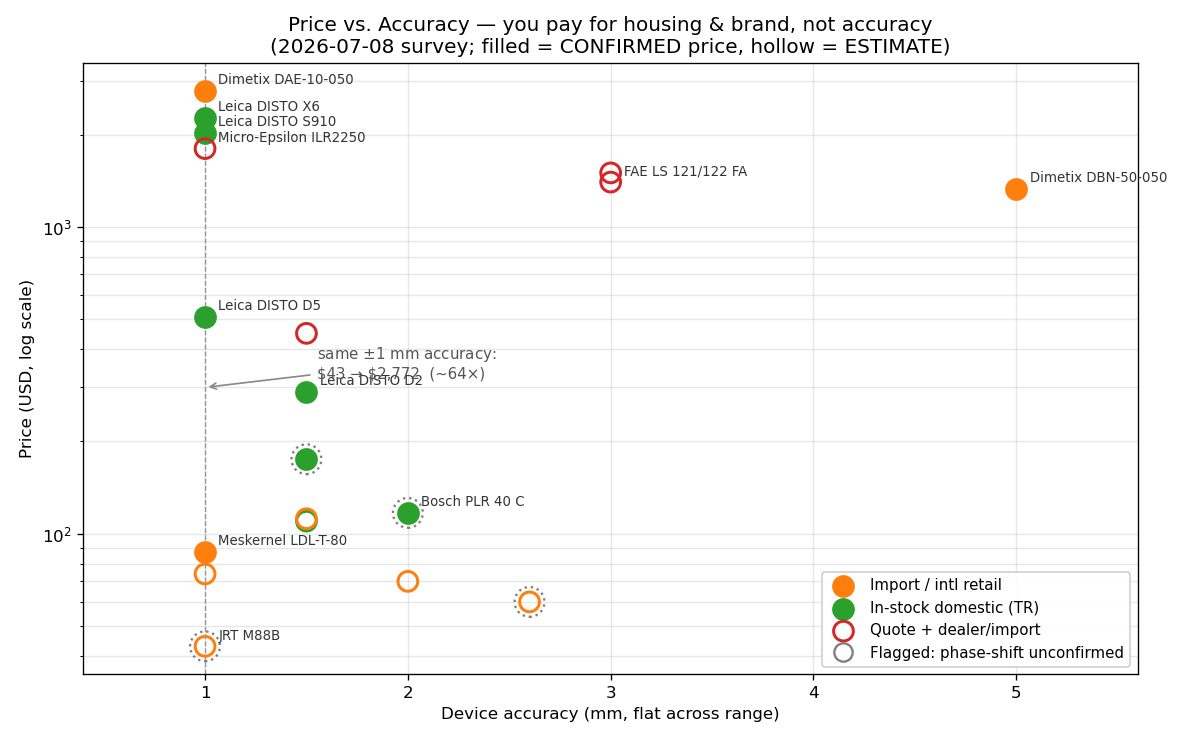
\includegraphics[height=0.80\textheight]{price_vs_accuracy.png}
\end{frame}

\begin{frame}{Turkey Sourcing --- Lead-Time by Availability Class}
  \centering
  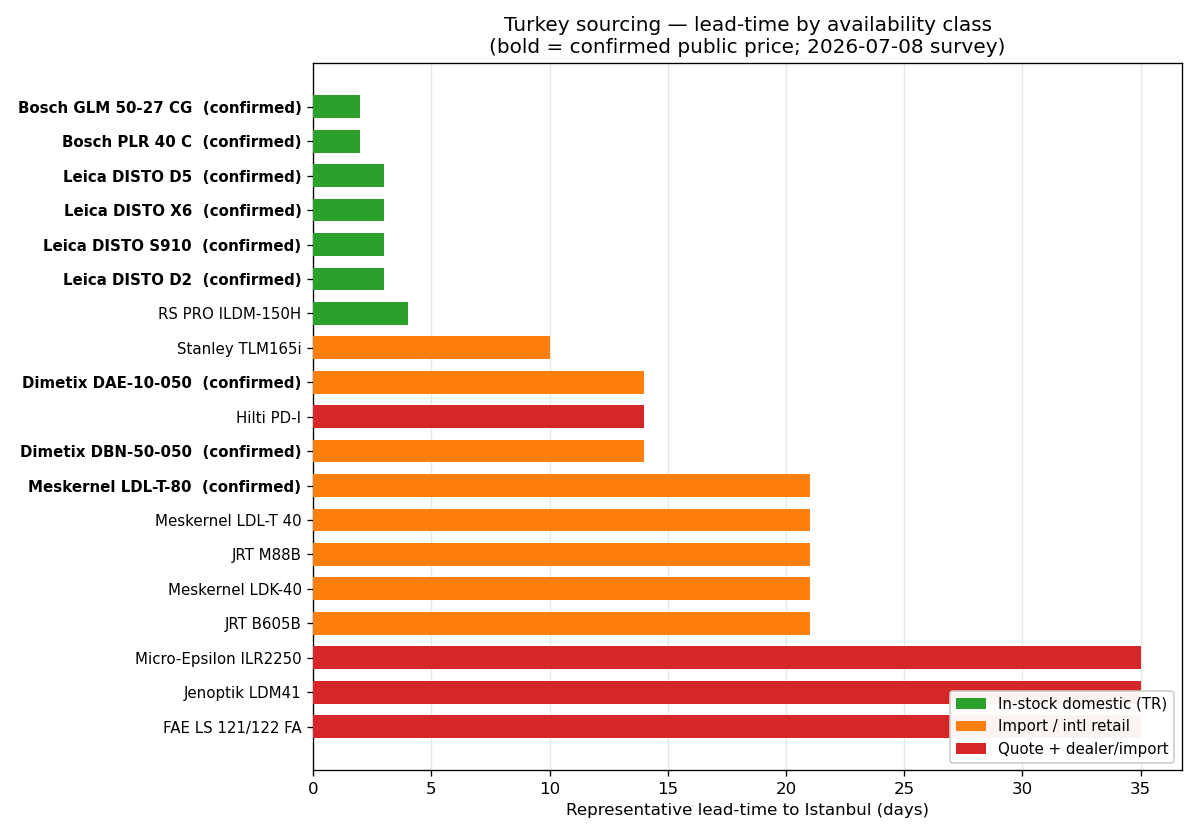
\includegraphics[height=0.80\textheight]{turkey_availability.png}
\end{frame}

% ---------------------------------------------------------------
\begin{frame}{Flagged: Attractive, but Principle Unconfirmed}
  The two cheapest/fastest options are \alert{held out of the certified list}:
  the 2026-07-08 survey could not confirm their measurement principle is
  phase-shift from any primary source. Verify before committing.
  \vspace{0.4em}

  \begin{columns}[c]
    \column{0.5\textwidth}
    \centering
    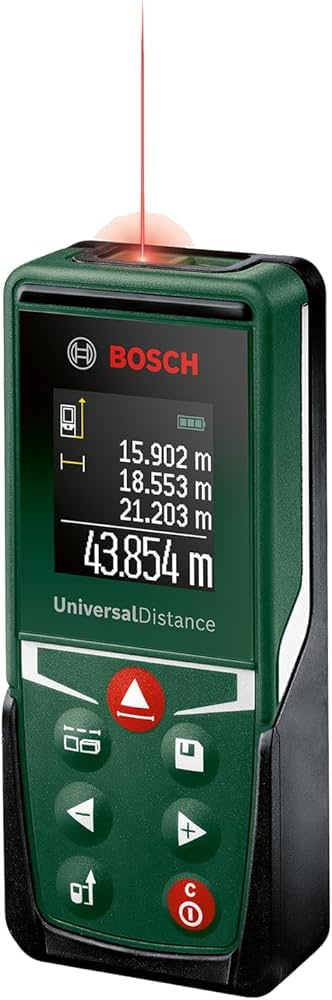
\includegraphics[height=3.8cm]{bosch_plr40c.jpg}\\[0.4em]
    \textbf{Bosch PLR 40 C}$^\dagger$\\
    \small $\pm$2 mm, best Turkey availability, BLE --- \alert{principle unconfirmed}.
    \column{0.5\textwidth}
    \centering
    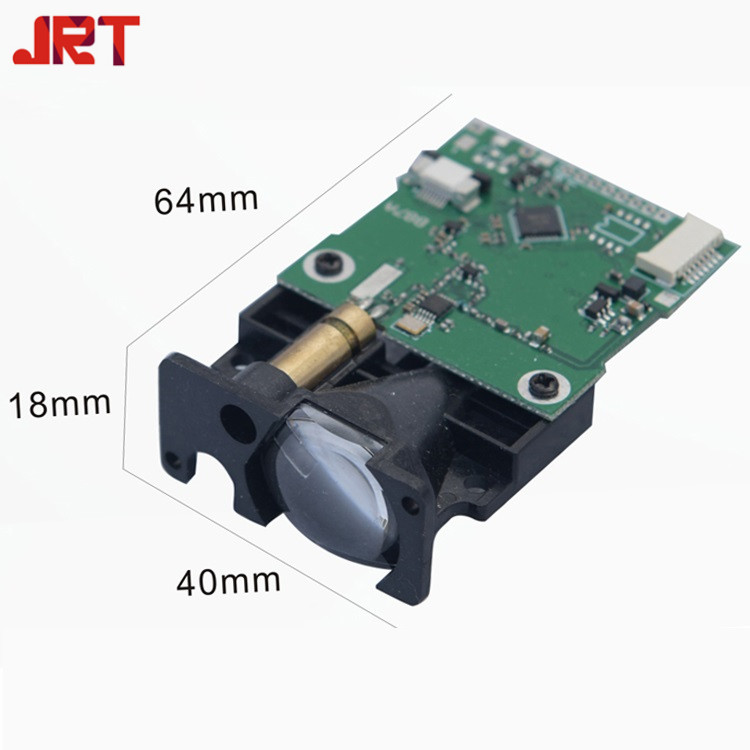
\includegraphics[height=3.8cm]{jrt_b605b.jpg}\\[0.4em]
    \textbf{JRT B605B}$^\dagger$\\
    \small Cheapest wired (\$43), docked (A) or fixed (B) --- \alert{principle unconfirmed}.
  \end{columns}
\end{frame}

% ---------------------------------------------------------------
\begin{frame}{Recommendation --- Bench-Test Order (confirmed-phase-shift first)}
  \begin{enumerate}
    \item \textbf{Meskernel LDL-T} --- order first. Cheapest device with confirmed
      phase-shift \emph{and} confirmed price (\$87.50); $\pm$1 mm, 100 Hz. Request the
      command datasheet before ordering.
    \item \textbf{Dimetix DBN-50-050} (\$1{,}332) --- the only \textbf{public ASCII protocol}
      in the study; de-risks the firmware parsing path. DAE-10-050 (\$2{,}700) for $\pm$1 mm.
    \item \textbf{Leica DISTO D5} (\$311--708, in TR) --- confirmed-phase-shift $\pm$1 mm
      handheld reference; clean BLE-path validation.
    \item \alert{Flagged} \textbf{Bosch / JRT / RS PRO} --- cheap \& fast, but only
      \emph{after} a datasheet confirms phase-shift. Industrial tier (ME / WayCon / FAE)
      only if certified housing is required.
  \end{enumerate}
\end{frame}

% ---------------------------------------------------------------
\begin{frame}{Context: System Error Budget (out of scope)}
  The $\leq$10 mm spec is the \emph{laser device} alone. The encoders' angular
  error \textbf{grows with range} --- past $\sim$15 m they dominate and
  \textbf{laser choice stops mattering} to total accuracy ($\approx$18 mm at 40 m).
  \vspace{-0.2em}
  \begin{center}
    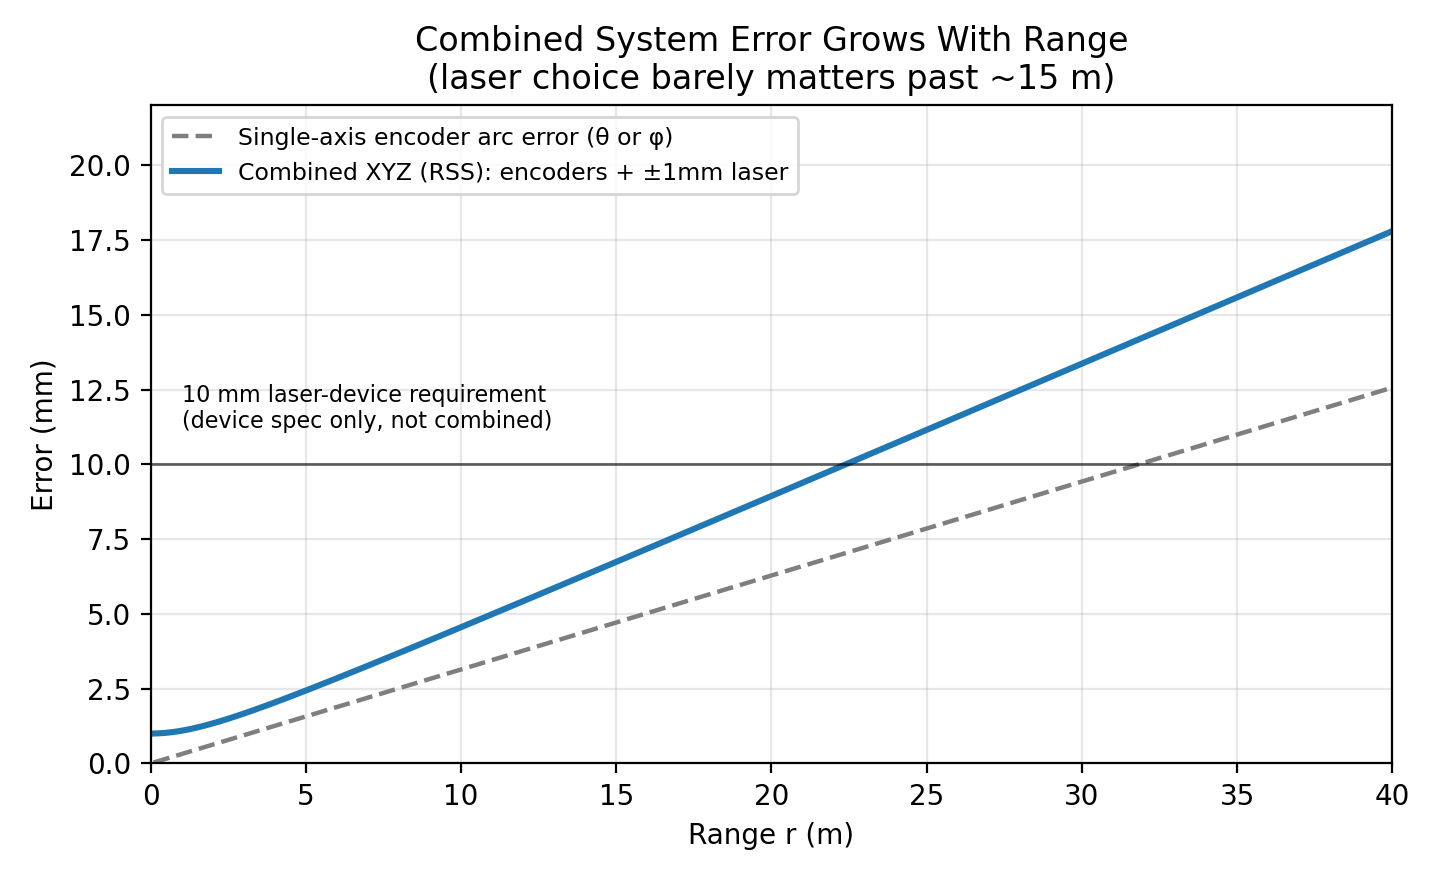
\includegraphics[height=0.66\textheight]{error_budget.png}
  \end{center}
\end{frame}

% ---------------------------------------------------------------
\begin{frame}[standout]{Conclusion}
  The $\leq$40 m / $\leq$10 mm requirement is \textbf{comfortably met} ---
  but only with phase-shift lasers.

  \vspace{0.8em}
  A cheap bench path (Bosch + RS PRO + JRT) validates the integration
  before spending on any industrial-grade unit.
\end{frame}

\end{document}
